% !TeX program = xelatex
% Generated locally. Edit slides/*.tex, or supply a reviewed layout JSON and rebuild.
\ifdefined\HandoutMode
  \documentclass[aspectratio=169,10pt,handout]{beamer}
\else
  \documentclass[aspectratio=169,10pt]{beamer}
\fi
\usepackage[UTF8,fontset=fandol]{ctex}
\IfFontExistsTF{Microsoft YaHei}{\setCJKsansfont{Microsoft YaHei}}{}
\usetheme{GaoZhongYuan}
\newcommand{\red}[1]{\textcolor{red}{#1}}
\setlength{\parskip}{.45em}
\begin{document}
\title{1.1.1 集合}\author{第一章  集合与逻辑}\date{}\campusmaketitle

\begin{frame}<1-4>[t]{学习目标}
\begin{campuscanvas}
% Source slide 2, objects 2; visible 2-4
\only<2-4|handout:1>{\node[anchor=north west,inner sep=0,text=black] at (70.000,200.000) {\begin{minipage}[t]{142.500mm}\raggedright\fontsize{14}{21.00}\selectfont \textcolor{campusgreen}{\textbf{01}}\quad 理解集合的含义，能判断给定对象能否构成集合。\end{minipage}};}
% Source slide 2, objects 15; visible 3-4
\only<3-4|handout:1>{\node[anchor=north west,inner sep=0,text=black] at (70.000,340.000) {\begin{minipage}[t]{142.500mm}\raggedright\fontsize{14}{21.00}\selectfont \textcolor{campusgreen}{\textbf{02}}\quad 掌握集合的常用表示方法，能根据集合特点选择合适方法表示集合。\end{minipage}};}
% Source slide 2, objects 18; visible 4
\only<4|handout:1>{\node[anchor=north west,inner sep=0,text=black] at (70.000,490.000) {\begin{minipage}[t]{142.500mm}\raggedright\fontsize{14}{21.00}\selectfont \textcolor{campusgreen}{\textbf{03}}\quad 熟知常见数集的记法，会用区间表示集合。\end{minipage}};}
\end{campuscanvas}
\end{frame}

\begin{frame}<1-5>[t]{新课导学}
\begin{campuscanvas}
% Source slide 3, objects 34; visible 2-5
\only<2-5|handout:1>{\node[anchor=north west,inner sep=0,text=black] at (70.000,145.000) {\begin{minipage}[t]{142.500mm}\raggedright\fontsize{12}{18.00}\selectfont 《三国志》记载：“布有良马曰赤兔。”据《三国演义》描述，这匹宝马后来跟随关羽并大展神威。\end{minipage}};}
% Source slide 3, objects 36; visible 3-5
\only<3-5|handout:1>{\node[anchor=north west,inner sep=0,text=black] at (70.000,275.000) {\begin{minipage}[t]{142.500mm}\raggedright\fontsize{12}{18.00}\selectfont \textbf{思考：}下面三句话里的“是”各自的含义是什么？\par A．关羽千里走单骑的坐骑是赤兔马。\par B．赤兔马是红马。\par C．红马是马。\end{minipage}};}
% Source slide 3, objects 3; visible 4-5
\only<4-5|handout:1>{\node[anchor=north west,inner sep=0,text=black] at (70.000,515.000) {\begin{minipage}[t]{142.500mm}\raggedright\fontsize{12}{18.00}\selectfont 第一个“是”的含义相当于“$=$”，另外两个呢？\end{minipage}};}
% Source slide 3, objects 8; visible 5
\only<5|handout:1>{\node[anchor=north west,inner sep=0,text=black] at (70.000,610.000) {\begin{minipage}[t]{142.500mm}\raggedright\fontsize{12}{18.00}\selectfont \red{B 中“是”表示属于，即赤兔马属于红马这一类别。}\end{minipage}};}
\end{campuscanvas}
\end{frame}

\begin{frame}<1-3>[t]{新知探索}
\begin{campuscanvas}
% Source slide 4, objects 25; visible 2-3
\only<2-3|handout:1>{\node[anchor=north west,inner sep=0,text=black] at (70.000,150.000) {\begin{minipage}[t]{142.500mm}\raggedright\fontsize{16}{24.00}\selectfont \textbf{1. 集合与元素概念}\end{minipage}};}
% Source slide 4, objects 24; visible 3
\only<3|handout:1>{\node[anchor=north west,inner sep=0,text=black] at (70.000,255.000) {\begin{minipage}[t]{142.500mm}\raggedright\fontsize{13}{19.50}\selectfont 我们在思考问题时，常常需要把一些对象放在一起考虑，并且给这些对象一个总的名称。\par 在数学语言中，把一些对象放在一起考虑时，就说这些对象组成了一个\red{集合}或\red{集}。这些对象的总的名称，就是这个集合的名字。\par 这些对象中的每一个，都叫作这个集合的一个\red{元素}。\end{minipage}};}
\end{campuscanvas}
\end{frame}

\begin{frame}<1-3>[t]{新知探索}
\begin{campuscanvas}
% Source slide 5, objects 2; visible 2-3
\only<2-3|handout:1>{\node[anchor=north west,inner sep=0,text=black] at (70.000,150.000) {\begin{minipage}[t]{142.500mm}\raggedright\fontsize{13}{19.50}\selectfont 例如，单词 element 中出现的字母组成一个集合，$e$ 是这个集合的一个元素；太阳系的八大行星组成一个集合，地球是这个集合的一个元素；所有大于 $2$ 的素数组成一个集合，$7$ 是这个集合的一个元素；等等。\end{minipage}};}
% Source slide 5, objects 4; visible 3
\only<3|handout:1>{\node[anchor=north west,inner sep=0] at (300.000,390.000) {
\includegraphics[width=85.000mm,height=35.375mm]{source-media/image12.png}};}
\end{campuscanvas}
\end{frame}

\begin{frame}<1-3>[t]{新知探索}
\begin{campuscanvas}
% Source slide 6, objects 9; visible 2-3
\only<2-3|handout:1>{\node[anchor=north west,inner sep=0,text=black] at (70.000,150.000) {\begin{minipage}[t]{142.500mm}\raggedright\fontsize{16}{24.00}\selectfont \textbf{2. 集合与元素的关系}\end{minipage}};}
% Source slide 6, objects 8; visible 3
\only<3|handout:1>{\node[anchor=north west,inner sep=0,text=black] at (70.000,260.000) {\begin{minipage}[t]{142.500mm}\raggedright\fontsize{13}{19.50}\selectfont 集合论中最基本的关系是集合和它的元素之间的归属关系。表达归属关系的符号是 $\in$，读作“\red{属于}”。\par 若 $S$ 是一个集合，$a$ 是 $S$ 的一个元素，记作 $a\in S$，读作“$a$ 属于 $S$”。\par 若 $a$ 不是集合 $S$ 的元素，记作 $a\notin S$，读作“$a$ \red{不属于} $S$”。\end{minipage}};}
\end{campuscanvas}
\end{frame}

\begin{frame}<1-3>[t]{新知探索}
\begin{campuscanvas}
% Source slide 7, objects 8; visible 2-3
\only<2-3|handout:1>{\node[anchor=north west,inner sep=0,text=black] at (70.000,190.000) {\begin{minipage}[t]{142.500mm}\raggedright\fontsize{14}{21.00}\selectfont \textbf{例 1}\quad 设 $L(A,B)$ 表示直线 $AB$ 上全体点组成的集合，$P\in L(A,B)$ 的含义是什么？\end{minipage}};}
% Source slide 7, objects 12; visible 3
\only<3|handout:1>{\node[anchor=north west,inner sep=0,text=black] at (70.000,390.000) {\begin{minipage}[t]{142.500mm}\raggedright\fontsize{14}{21.00}\selectfont \red{解}\quad $P\in L(A,B)$ 表示“$P$ 是直线 $AB$ 上的一个点”。\end{minipage}};}
\end{campuscanvas}
\end{frame}

\begin{frame}<1-5>[t]{新知探索}
\begin{campuscanvas}
% Source slide 8, objects 5; visible 1-5
\only<1-5|handout:1>{\node[anchor=north west,inner sep=0,text=black] at (70.000,150.000) {\begin{minipage}[t]{142.500mm}\raggedright\fontsize{14}{21.00}\selectfont \textbf{思考}\quad 军训时教官喊 13 班集合：\end{minipage}};}
% Source slide 8, objects 8; visible 2-5
\only<2-5|handout:1>{\node[anchor=north west,inner sep=0,text=black] at (70.000,255.000) {\begin{minipage}[t]{100.000mm}\raggedright\fontsize{12}{18.00}\selectfont 14 班学生会不会跑到 13 班来？\end{minipage}};}
% Source slide 8, objects 8; visible 2-5
\only<2-5|handout:1>{\node[anchor=north west,inner sep=0,text=black] at (70.000,360.000) {\begin{minipage}[t]{100.000mm}\raggedright\fontsize{12}{18.00}\selectfont 教官调整了站位后班级里的人有没有发生变化？\par 班级会不会发生改变？\end{minipage}};}
% Source slide 8, objects 8; visible 2-5
\only<2-5|handout:1>{\node[anchor=north west,inner sep=0,text=black] at (70.000,535.000) {\begin{minipage}[t]{100.000mm}\raggedright\fontsize{12}{18.00}\selectfont 教官要求报数的目的是什么？一个人是否会报两次？\end{minipage}};}
% Source slide 8, objects 9; visible 3-5
\only<3-5|handout:1>{\node[anchor=north west,inner sep=0,text=black] at (970.000,255.000) {\begin{minipage}[t]{28.750mm}\raggedright\fontsize{14}{21.00}\selectfont \red{确定性}\end{minipage}};}
% Source slide 8, objects 11; visible 4-5
\only<4-5|handout:1>{\node[anchor=north west,inner sep=0,text=black] at (970.000,380.000) {\begin{minipage}[t]{28.750mm}\raggedright\fontsize{14}{21.00}\selectfont \red{无序性}\end{minipage}};}
% Source slide 8, objects 12; visible 5
\only<5|handout:1>{\node[anchor=north west,inner sep=0,text=black] at (970.000,545.000) {\begin{minipage}[t]{28.750mm}\raggedright\fontsize{14}{21.00}\selectfont \red{互异性}\end{minipage}};}
\end{campuscanvas}
\end{frame}

\begin{frame}<1-2>[t]{新知探索}
\begin{campuscanvas}
% Source slide 9, objects 11; visible 1-2
\only<1-2|handout:1>{\node[anchor=north west,inner sep=0,text=black] at (70.000,150.000) {\begin{minipage}[t]{142.500mm}\raggedright\fontsize{16}{24.00}\selectfont \textbf{3. 元素的性质}\end{minipage}};}
% Source slide 9, objects 2,5; visible 1-2
\only<1-2|handout:1>{\node[anchor=north west,inner sep=0,text=black] at (70.000,245.000) {\begin{minipage}[t]{142.500mm}\raggedright\fontsize{12}{18.00}\selectfont \red{1. 确定性：}对于一个给定的集合，它的元素必须是确定的。也就是说，对于一个已知的集合来说，某个元素在不在这个集合里，是确定的，要么在，要么不在，不能含糊其辞。\end{minipage}};}
% Source slide 9, objects 4,6; visible 1-2
\only<1-2|handout:1>{\node[anchor=north west,inner sep=0,text=black] at (70.000,410.000) {\begin{minipage}[t]{142.500mm}\raggedright\fontsize{12}{18.00}\selectfont \red{2. 无序性：}集合中的元素无先后顺序。\end{minipage}};}
% Source slide 9, objects 7,8; visible 1-2
\only<1-2|handout:1>{\node[anchor=north west,inner sep=0,text=black] at (70.000,490.000) {\begin{minipage}[t]{142.500mm}\raggedright\fontsize{12}{18.00}\selectfont \red{3. 互异性：}集合中的元素必须互不相同。\end{minipage}};}
% Source slide 9, objects 9; visible 2
\only<2|handout:1>{\node[anchor=north west,inner sep=0,text=black] at (70.000,580.000) {\begin{minipage}[t]{142.500mm}\raggedright\fontsize{12}{18.00}\selectfont \textbf{集合相等：}只要构成两个集合的元素\red{一样}，我们就称这两个集合是\red{相等}的。\end{minipage}};}
\end{campuscanvas}
\end{frame}

\begin{frame}<1-3>[t]{新知探索}
\begin{campuscanvas}
% Source slide 10, objects 9; visible 2-3
\only<2-3|handout:1>{\node[anchor=north west,inner sep=0,text=black] at (70.000,150.000) {\begin{minipage}[t]{142.500mm}\raggedright\fontsize{16}{24.00}\selectfont \textbf{4. 常见数集及分类}\end{minipage}};}
% Source slide 10, objects 13; visible 3
\only<3|handout:1>{\node[anchor=north west,inner sep=0,text=black] at (70.000,260.000) {\begin{minipage}[t]{142.500mm}\raggedright\fontsize{13}{19.50}\selectfont 数学里最常用的集合是各种数的集合，简称数集。例如：\par 全体自然数组成的集合叫\red{自然数集}，记作 $\mathbf N$。\par 全体整数组成的集合叫\red{整数集}，记作 $\mathbf Z$。\par 全体有理数组成的集合叫\red{有理数集}，记作 $\mathbf Q$。\par 全体实数组成的集合叫\red{实数集}，记作 $\mathbf R$。\end{minipage}};}
\end{campuscanvas}
\end{frame}

\begin{frame}<1-2>[t]{新知探索}
\begin{campuscanvas}
% Source slide 11, objects 2; visible 2
\only<2|handout:1>{\node[anchor=north west,inner sep=0,text=black] at (70.000,195.000) {\begin{minipage}[t]{142.500mm}\raggedright\fontsize{13}{19.50}\selectfont 通常用 $\mathbf R_+$ 表示全体正实数组成的集合；类似的有\[\mathbf R_-,\quad\mathbf Z_+,\quad\mathbf N_+,\quad\mathbf Q_-,\quad\cdots.\]\par 元素个数有限的集合叫\red{有限集}（或有穷集），元素无限多的集合叫\red{无限集}（或无穷集）。\par 没有元素的集合叫\red{空集}，记作 $\varnothing$；\textbf{空集也是有限集}。\end{minipage}};}
\end{campuscanvas}
\end{frame}

\begin{frame}<1-4>[t]{新知探索}
\begin{campuscanvas}
% Source slide 12, objects 12; visible 2-4
\only<2-4|handout:1>{\node[anchor=north west,inner sep=0,text=black] at (70.000,150.000) {\begin{minipage}[t]{140.000mm}\raggedright\fontsize{12}{18.00}\selectfont \textbf{例 2}\quad 下列集合中哪些是有限集？哪些是无限集？\par （1）一元二次方程 $x^2+1=0$ 的全体实数根组成的集合；\par （2）所有素数组成的集合；\par （3）所有矩形组成的集合；\par （4）所有亚洲国家组成的集合。\end{minipage}};}
% Source slide 12, objects 17; visible 3-4
\only<3-4|handout:1>{\node[anchor=north west,inner sep=0,text=black] at (70.000,425.000) {\begin{minipage}[t]{142.500mm}\raggedright\fontsize{11}{16.50}\selectfont \textcolor{campusgreen}{\textbf{素数}}\quad 如果一个大于 $1$ 的整数，除 $1$ 和自身外无其他正因数，则称这个正整数为素数。\end{minipage}};}
% Source slide 12, objects 14; visible 4
\only<4|handout:1>{\node[anchor=north west,inner sep=0,text=black] at (70.000,550.000) {\begin{minipage}[t]{142.500mm}\raggedright\fontsize{11}{16.50}\selectfont \red{解}\quad （1）$x^2+1=0$ 没有实根，故为空集，是有限集。\par （2）（3）素数和矩形均有无穷多个，是无限集。\par （4）亚洲国家的个数有限，是有限集。\end{minipage}};}
\end{campuscanvas}
\end{frame}

\begin{frame}<1-4>[t]{新知探索}
\begin{campuscanvas}
% Source slide 13, objects 25; visible 2-4
\only<2-4|handout:1>{\node[anchor=north west,inner sep=0,text=black] at (70.000,150.000) {\begin{minipage}[t]{142.500mm}\raggedright\fontsize{16}{24.00}\selectfont \textbf{5. 表示集合的方法：列举法}\end{minipage}};}
% Source slide 13, objects 24; visible 3-4
\only<3-4|handout:1>{\node[anchor=north west,inner sep=0,text=black] at (70.000,245.000) {\begin{minipage}[t]{142.500mm}\raggedright\fontsize{12}{18.00}\selectfont 表示一个集合，就是把它有哪些元素交代清楚。生活中常见的方法，是\red{把集合中的元素一一列举出来}。\par 饭馆里的菜单，计算机里的文件夹，各种委员会名单，都是这样做的。这种表示法叫作\red{列举法}。\end{minipage}};}
% Source slide 13, objects 5; visible 4
\only<4|handout:1>{\node[anchor=north west,inner sep=0,text=black] at (70.000,475.000) {\begin{minipage}[t]{142.500mm}\raggedright\fontsize{12}{18.00}\selectfont 数学里用列举法表示集合，常用的格式是在一个大括号里写出每个元素的名字，相邻的名字用逗号分隔。\par 例如，小于 $10$ 的正偶数组成的集合，用列举法可以表示为\[\{2,4,6,8\}\quad\text{或}\quad\{8,2,6,4\}\quad\text{等。}\]\end{minipage}};}
\end{campuscanvas}
\end{frame}

\begin{frame}<1-3>[t]{新知探索}
\begin{campuscanvas}
% Source slide 14, objects 2; visible 2-3
\only<2-3|handout:1>{\node[anchor=north west,inner sep=0,text=black] at (70.000,170.000) {\begin{minipage}[t]{142.500mm}\raggedright\fontsize{13}{19.50}\selectfont \textbf{例 3}\quad 用列举法表示下列集合：\par （1）由方程 $x^2-1=0$ 的所有实数解构成的集合 $S$；\par （2）平方小于 $225$ 的所有素数构成的集合 $P$。\end{minipage}};}
% Source slide 14, objects 10; visible 3
\only<3|handout:1>{\node[anchor=north west,inner sep=0,text=black] at (70.000,395.000) {\begin{minipage}[t]{142.500mm}\raggedright\fontsize{13}{19.50}\selectfont \red{解}\quad （1）$S=\{1,-1\}$。\par （2）平方小于 $225$ 的正整数有 $1,2,3,\ldots,14$，于是\[P=\{2,3,5,7,11,13\}.\]\end{minipage}};}
\end{campuscanvas}
\end{frame}

\begin{frame}<1-3>[t]{新知探索}
\begin{campuscanvas}
% Source slide 15, objects 25; visible 2-3
\only<2-3|handout:1>{\node[anchor=north west,inner sep=0,text=black] at (70.000,150.000) {\begin{minipage}[t]{142.500mm}\raggedright\fontsize{16}{24.00}\selectfont \textbf{6. 表示集合的方法：描述法}\end{minipage}};}
% Source slide 15, objects 24; visible 3
\only<3|handout:1>{\node[anchor=north west,inner sep=0,text=black] at (70.000,250.000) {\begin{minipage}[t]{142.500mm}\raggedright\fontsize{13}{19.50}\selectfont 无限集一般不能用列举法表示。有限集如果元素太多或叫不出名字来，例如某池塘里所有鱼的集合，也不便用列举法来表示。\par 这时可以\red{把集合中元素共有的，也只有该集合中元素才有的属性描述出来，以确定这个集合}。这种表示法叫作\red{描述法}。\par 集会时介绍嘉宾常用列举法，致辞里说“女士们，先生们”用的就是描述法。\end{minipage}};}
\end{campuscanvas}
\end{frame}

\begin{frame}<1-3>[t]{新知探索}
\begin{campuscanvas}
% Source slide 16, objects 9; visible 2-3
\only<2-3|handout:1>{\node[anchor=north west,inner sep=0,text=black] at (70.000,150.000) {\begin{minipage}[t]{142.500mm}\raggedright\fontsize{16}{24.00}\selectfont \textbf{描述法表示集合的格式}\end{minipage}};}
% Source slide 16, objects 2; visible 3
\only<3|handout:1>{\node[anchor=north west,inner sep=0,text=black] at (70.000,235.000) {\begin{minipage}[t]{142.500mm}\raggedright\fontsize{11.5}{17.25}\selectfont 在一个大括号里写出集合中元素的共有属性。例如，集合 $\{2,4,6,8\}$ 可表示为 $\{\text{小于 10 的正偶数}\}$。\par 将“红马”看作集合，可表示为 $\{\text{红马}\}$，“赤兔马是红马”可表示为“赤兔马 $\in\{\text{红马}\}$”，这里的“是”相当于“$\in$”。\par 若用一句话描述不方便，通常先写出集合元素的一般属性或形式，再画一条竖线，竖线后列出元素要满足的条件。\par 例如，任何偶数都可表示为 $x=2k,\ k\in\mathbf Z$，所有偶数的集合为\[E=\{x\in\mathbf Z\mid x=2k,\ k\in\mathbf Z\}.\]\end{minipage}};}
\end{campuscanvas}
\end{frame}

\begin{frame}<1-3>[t]{新知探索}
\begin{campuscanvas}
% Source slide 17, objects 2; visible 2-3
\only<2-3|handout:1>{\node[anchor=north west,inner sep=0,text=black] at (70.000,150.000) {\begin{minipage}[t]{142.500mm}\raggedright\fontsize{12.5}{18.75}\selectfont \textbf{例 4}\quad 选择适当方法表示下列集合：\par （1）由大于 $20$ 且小于 $30$ 的所有实数组成的集合 $A$；\par （2）由方程 $x^2+y^2=4$ 的所有整数解 $(x,y)$ 组成的集合 $B$。\end{minipage}};}
% Source slide 17, objects 4; visible 3
\only<3|handout:1>{\node[anchor=north west,inner sep=0,text=black] at (70.000,395.000) {\begin{minipage}[t]{142.500mm}\raggedright\fontsize{12}{18.00}\selectfont \red{解}\quad （1）用描述法：$A=\{x\in\mathbf R\mid 20<x<30\}$。\par （2）用列举法：$B=\{(0,2),(0,-2),(2,0),(-2,0)\}$。\par 用描述法：$B=\{(x,y)\mid x^2+y^2=4,\ x\in\mathbf Z,\ y\in\mathbf Z\}$。\end{minipage}};}
\end{campuscanvas}
\end{frame}

\begin{frame}<1-4>[t]{新知探索}
\begin{campuscanvas}
% Source slide 18, objects 10; visible 2-4
\only<2-4|handout:1>{\node[anchor=north west,inner sep=0,text=black] at (70.000,150.000) {\begin{minipage}[t]{142.500mm}\raggedright\fontsize{16}{24.00}\selectfont \textbf{7. 区间}\end{minipage}};}
% Source slide 18, objects 8; visible 3-4
\only<3-4|handout:1>{\node[anchor=north west,inner sep=0,text=black] at (70.000,235.000) {\begin{minipage}[t]{103.750mm}\raggedright\fontsize{11.5}{17.25}\selectfont 数学里最常用的一类集合叫\red{区间}。\par 设 $a,b\in\mathbf R$，且 $a<b$。\par 所有大于 $a$ 且小于 $b$ 的实数组成\red{开区间}：\[(a,b)=\{x\in\mathbf R\mid a<x<b\}.\]满足 $a\le x\le b$ 的实数组成\red{闭区间} $[a,b]$。\par 类似地，还有左开右闭区间 $(a,b]$ 和左闭右开区间 $[a,b)$。$a,b$ 分别是区间的\red{左端点}和\red{右端点}。\end{minipage}};}
% Source slide 18, objects 9; visible 4
\only<4|handout:1>{\node[anchor=north west,inner sep=0] at (940.000,280.000) {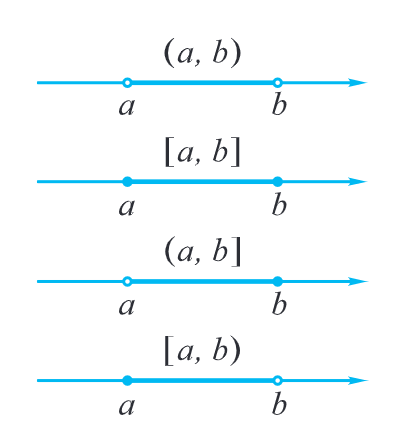
\includegraphics[width=35.000mm,height=40.625mm]{source-media/image26.png}};}
\end{campuscanvas}
\end{frame}

\begin{frame}<1-2>[t]{新知探索}
\begin{campuscanvas}
% Source slide 19, objects 2; visible 2
\only<2|handout:1>{\node[anchor=north west,inner sep=0,text=black] at (70.000,190.000) {\begin{minipage}[t]{142.500mm}\raggedright\fontsize{13}{19.50}\selectfont 实数集 $\mathbf R$ 可以用区间表示为 $(-\infty,+\infty)$。符号 $\infty$ 读作“无穷大”或“无穷”；$-\infty$ 和 $+\infty$ 分别读作“负无穷大”和“正无穷大”。\par 满足条件 $x\ge a$、$x>a$、$x\le b$、$x<b$ 的实数 $x$ 的集合分别为\[\begin{aligned}x\ge a&:\quad [a,+\infty),&x>a&:\quad (a,+\infty),\\[1em]x\le b&:\quad (-\infty,b],&x<b&:\quad (-\infty,b).\end{aligned}\]\end{minipage}};}
\end{campuscanvas}
\end{frame}

\begin{frame}<1-4>[t]{例题讲解}
\begin{campuscanvas}
% Source slide 20, objects 2; visible 2-4
\only<2-4|handout:1>{\node[anchor=north west,inner sep=0,text=black] at (70.000,155.000) {\begin{minipage}[t]{98.750mm}\raggedright\fontsize{12}{18.00}\selectfont \textbf{例 5}\quad 用区间表示下列集合：\par （1）$\{x\in\mathbf R\mid -2\le x\le4\}$；\par （2）$\{t\in\mathbf R\mid t<a,\ a\in\mathbf R\}$；\par （3）$\{u\in\mathbf R\mid u\ge0\}$。\end{minipage}};}
% Source slide 20, objects 4; visible 3-4
\only<3-4|handout:1>{\node[anchor=north west,inner sep=0,text=black] at (70.000,420.000) {\begin{minipage}[t]{142.500mm}\raggedright\fontsize{12}{18.00}\selectfont \red{解}\quad （1）$\{x\in\mathbf R\mid -2\le x\le4\}=[-2,4]$；\par （2）$\{t\in\mathbf R\mid t<a,\ a\in\mathbf R\}=(-\infty,a)$；\par （3）$\{u\in\mathbf R\mid u\ge0\}=[0,+\infty)$。\end{minipage}};}
% Source slide 20, objects 32; visible 4
\only<4|handout:1>{\node[anchor=north west,inner sep=0,text=black] at (915.000,155.000) {\begin{minipage}[t]{37.500mm}\raggedright\fontsize{9.5}{14.25}\selectfont \textcolor{campusgreen}{\textbf{约定}}\par 如果从上下文的关系看，$x\in\mathbf R$ 是明确的，那么集合 $\{x\in\mathbf R\mid x<4\}$ 可简写为 $\{x\mid x<4\}$。\end{minipage}};}
\end{campuscanvas}
\end{frame}

\begin{frame}<1-4>[t]{课堂巩固}
\begin{campuscanvas}
% Source slide 21, objects 8; visible 2-4
\only<2-4|handout:1>{\node[anchor=north west,inner sep=0,text=black] at (70.000,155.000) {\begin{minipage}[t]{142.500mm}\raggedright\fontsize{12.5}{18.75}\selectfont \textbf{1.} 下面给出的四类对象中，能构成集合的是（\quad）。\par A．某班视力较好的同学\qquad B．某小区长寿的人\par C．$\pi$ 的近似值\qquad\qquad D．方程 $x^2=1$ 的实数根\end{minipage}};}
% Source slide 21, objects 10; visible 3-4
\only<3-4|handout:1>{\node[anchor=north west,inner sep=0,text=black] at (70.000,355.000) {\begin{minipage}[t]{142.500mm}\raggedright\fontsize{14}{21.00}\selectfont \red{\textbf{答案：D}}\end{minipage}};}
% Source slide 21, objects 9; visible 4
\only<4|handout:1>{\node[anchor=north west,inner sep=0,text=black] at (70.000,445.000) {\begin{minipage}[t]{142.500mm}\raggedright\fontsize{11.5}{17.25}\selectfont \red{解析：}\par A．“视力较好”不确定，不能构成集合。\par B．“长寿”不确定，不能构成集合。\par C．未给出精确度，“$\pi$ 的近似值”不确定，不能构成集合。\par D．方程 $x^2=1$ 的实数根是 $-1$ 和 $1$，明确可靠，能构成集合。故选 D。\end{minipage}};}
\end{campuscanvas}
\end{frame}

\begin{frame}<1-4>[t]{课堂巩固}
\begin{campuscanvas}
% Source slide 22, objects 2; visible 2-4
\only<2-4|handout:1>{\node[anchor=north west,inner sep=0,text=black] at (70.000,155.000) {\begin{minipage}[t]{142.500mm}\raggedright\fontsize{13}{19.50}\selectfont \textbf{2.} 下列关系中，正确的是（\quad）。\par A．$-2\in\mathbf N_+$\qquad\qquad B．$\dfrac32\in\mathbf Z$\par C．$\pi\notin\mathbf Q$\qquad\qquad D．$5\notin\mathbf N$\end{minipage}};}
% Source slide 22, objects 10; visible 3-4
\only<3-4|handout:1>{\node[anchor=north west,inner sep=0,text=black] at (70.000,365.000) {\begin{minipage}[t]{142.500mm}\raggedright\fontsize{14}{21.00}\selectfont \red{\textbf{答案：C}}\end{minipage}};}
% Source slide 22, objects 13; visible 4
\only<4|handout:1>{\node[anchor=north west,inner sep=0,text=black] at (70.000,445.000) {\begin{minipage}[t]{142.500mm}\raggedright\fontsize{11}{16.50}\selectfont \red{解析：}\par A．$-2$ 是负整数，$-2\notin\mathbf N_+$，错误。\par B．$\dfrac32$ 是分数，$\dfrac32\notin\mathbf Z$，错误。\par C．$\pi$ 是无理数，$\pi\notin\mathbf Q$，正确。\par D．$5$ 是正整数，$5\in\mathbf N$，错误。故选 C。\end{minipage}};}
\end{campuscanvas}
\end{frame}

\begin{frame}<1-3>[t]{课堂巩固}
\begin{campuscanvas}
% Source slide 23, objects 8; visible 2-3
\only<2-3|handout:1>{\node[anchor=north west,inner sep=0,text=black] at (70.000,175.000) {\begin{minipage}[t]{142.500mm}\raggedright\fontsize{13}{19.50}\selectfont \textbf{3.} 下列选项中集合 $M,N$ 表示同一集合的是（\quad）。\par A．$M=\{3,4\},\quad N=\{4,3\}$\par B．$M=\{(3,4)\},\quad N=\{(4,3)\}$\par C．$M=\{(x,y)\mid x+y=4\},\quad N=\{y\mid x+y=4\}$\par D．$M=\{4,3\},\quad N=\{(4,3)\}$\end{minipage}};}
% Source slide 23, objects 9; visible 3
\only<3|handout:1>{\node[anchor=north west,inner sep=0,text=black] at (70.000,560.000) {\begin{minipage}[t]{142.500mm}\raggedright\fontsize{15}{22.50}\selectfont \red{\textbf{答案：A}}\end{minipage}};}
\end{campuscanvas}
\end{frame}

\begin{frame}<1-2>[t]{课堂巩固}
\begin{campuscanvas}
% Source slide 24, objects 3; visible 2
\only<2|handout:1>{\node[anchor=north west,inner sep=0,text=black] at (70.000,190.000) {\begin{minipage}[t]{142.500mm}\raggedright\fontsize{13}{19.50}\selectfont \red{解析：}\par A．根据集合元素的无序性，可得 $M=N$，正确。\par B．$(3,4)$ 和 $(4,3)$ 是不同的元素，错误。\par C．$M$ 中的元素是有序实数对，$N$ 中的元素是实数，错误。\par D．$M$ 中有两个元素，即 $4,3$；$N$ 中只有一个元素，即 $(4,3)$，错误。\par 故选 A。\end{minipage}};}
\end{campuscanvas}
\end{frame}

\begin{frame}<1-4>[t]{课堂巩固}
\begin{campuscanvas}
% Source slide 25, objects 8; visible 2-4
\only<2-4|handout:1>{\node[anchor=north west,inner sep=0,text=black] at (70.000,155.000) {\begin{minipage}[t]{142.500mm}\raggedright\fontsize{12.5}{18.75}\selectfont \textbf{4.} 已知集合 $A=\{1,2,3,4,5\}$，\[B=\{(x,y)\mid x\in A,\ y\in A,\ x-y\in A\},\]则 $B$ 中所含元素的个数为（\quad）。\par A．$3$\qquad B．$6$\qquad C．$8$\qquad D．$10$\end{minipage}};}
% Source slide 25, objects 9; visible 3-4
\only<3-4|handout:1>{\node[anchor=north west,inner sep=0,text=black] at (70.000,440.000) {\begin{minipage}[t]{142.500mm}\raggedright\fontsize{14}{21.00}\selectfont \red{\textbf{答案：D}}\end{minipage}};}
% Source slide 25, objects 11; visible 4
\only<4|handout:1>{\node[anchor=north west,inner sep=0,text=black] at (70.000,530.000) {\begin{minipage}[t]{142.500mm}\raggedright\fontsize{12}{18.00}\selectfont \red{解析：}\quad 当 $x=1$ 时，不存在符合条件的 $y$；\par 当 $x=2,3,4,5$ 时，符合条件的 $y$ 分别有 $1,2,3,4$ 个。\par 所以 $B$ 中所含元素的个数为 $1+2+3+4=10$。故选 D。\end{minipage}};}
\end{campuscanvas}
\end{frame}

\begin{frame}<1-3>[t]{课堂巩固}
\begin{campuscanvas}
% Source slide 26, objects 3; visible 2-3
\only<2-3|handout:1>{\node[anchor=north west,inner sep=0,text=black] at (70.000,155.000) {\begin{minipage}[t]{142.500mm}\raggedright\fontsize{12}{18.00}\selectfont \textbf{5.} 用符号“$\in$”或“$\notin$”填空：\par （1）$0\ \underline{\qquad}\ \varnothing$；\qquad（2）$-2\ \underline{\qquad}\ \{x\mid x^2<5\}$；\par （3）$(2,3)\ \underline{\qquad}\ \{(x,y)\mid x+2y=3\}$；\par （4）$2017\ \underline{\qquad}\ \{x\mid x=4n-1,\ n\in\mathbf Z\}$。\end{minipage}};}
% Source slide 26, objects 4; visible 3
\only<3|handout:1>{\node[anchor=north west,inner sep=0,text=black] at (70.000,405.000) {\begin{minipage}[t]{142.500mm}\raggedright\fontsize{11.5}{17.25}\selectfont \red{答案：}\quad （1）$\notin$\quad （2）$\in$\quad （3）$\notin$\quad （4）$\notin$。\par \red{解析：}\quad （1）空集不含任何元素，所以 $0\notin\varnothing$。\par （2）$(-2)^2=4<5$，所以 $-2\in\{x\mid x^2<5\}$。\par （3）$2+2\times3=8\ne3$，所以 $(2,3)\notin\{(x,y)\mid x+2y=3\}$。\par （4）$2017$ 不能表示为 $4n-1\ (n\in\mathbf Z)$，所以不属于该集合。\end{minipage}};}
\end{campuscanvas}
\end{frame}

\begin{frame}<1-2>[t]{课堂总结}
\begin{campuscanvas}
% Source slide 27, objects 13; visible 2
\only<2|handout:1>{\node[anchor=north west,inner sep=0,text=black] at (280.000,240.000) {\begin{minipage}[t]{100.000mm}\raggedright\fontsize{17}{25.50}\selectfont \textbf{1.} 集合的概念\par \textbf{2.} 集合的表示方法\par \textbf{3.} 常见数集\par \textbf{4.} 区间\end{minipage}};}
\end{campuscanvas}
\end{frame}

\campusclosing[谢谢观看]

\end{document}
